\documentclass[11pt,letterpaper]{article}

% Load some basic packages that are useful to have
% and that should be part of any LaTeX installation.
%
% be able to include figures
\usepackage{graphicx}
% get nice colors
\usepackage{xcolor}

% change default font to Palatino (looks nicer!)
\usepackage[latin1]{inputenc}
\usepackage{mathpazo}
\usepackage[T1]{fontenc}
% load some useful math symbols/fonts
\usepackage{latexsym,amsfonts,amsmath,amssymb}

% comfort package to easily set margins
\usepackage[top=1in, bottom=1in, left=1in, right=1in]{geometry}

\usepackage{courier}

% control some spacings
%
% spacing after a paragraph
\setlength{\parskip}{.15cm}
% indentation at the top of a new paragraph
\setlength{\parindent}{0.0cm}


\begin{document}

\begin{center}
\Large
Ay190 -- Final Project\\
Scott Barenfeld\\
D\'{o}nal O Sullivan\\
Date: \today
\end{center}

\section{Introduction}
Radio interferometers allow information from multiple radio antennae to be 
combined, giving the interferometer as a whole much greater resolution than 
a single dish on its own.  Because radio telescopes measure the incoming 
electric field itself (as a voltage), instead of just its intensity, the 
amplitude and phase of the electric field is preserved.  In an array, the 
time-averaged product of the voltages measured by each pair of antennae is 
reported as a \emph{visibility}.  Between antennas $i$ and $j$, the 
visibility is defined as:

\begin{equation}\label{eq:vis}
\mathcal{V}=\int_{4\pi} \! A(\hat{r})I(\hat{r})e^{-2\pi i\nu\vec{B}\cdot\hat{r}/c} \, \mathrm{d}\Omega,
\end{equation} 

where $A$ is the beam pattern of an individual antenna (in this case, a Gaussian 
with $\sigma$=1 arcmin), $I$ is the intensity 
of the sky, $\nu$ is the frequency of the radiation, $\vec{B}$ is the baseline 
vector between $i$ and $j$ ($\vec{r_i}-\vec{r_j}$), and $\hat{r}$ is the 
direction along the line of sight.  In the limit of a narrow field of view, 
Equation \ref{eq:vis} can be rewritten using a change of variables as: 

\begin{equation}\label{eq:vis2}
\mathcal{V}(u,v)=\int_{-\infty}^{\infty} \! \int_{-\infty}^{\infty} \! \frac{A(l,m)I(l,m)}{\sqrt{1-l^2-m^2}}e^{-2\pi i(ul+vm)} \, \mathrm{d}l \, \mathrm{d}m,
\end{equation}
where $(u,v)$ is the baseline vector between the two antennae in units of 
wavelengths and $l$ and $m$ are the angles (in radians) on the sky relative 
to the line of sight.  Equation \ref{eq:vis2} is simply a two-dimensional 
Fourier transform.  Thus, an image of the intensity pattern on the sky can 
be generated from the inverse Fourier transform of the measured visibilities.

\begin{equation}\label{eq:vis3}
\frac{I(l,m)A(l,m)}{\sqrt{1-l^2-m^2}}=\int_{-\infty}^{\infty} \! \int_{-\infty}^{\infty} \! \mathcal{V}(u,v)e^{2\pi i(ul+vm)} \, \mathrm{d}u \, \mathrm{d}v,
\end{equation}  

\section{Setup}
For this project, Michael provided us with a list of antenna positions and a 
list of the amplitude and phase of the visibility for each antenna pair, such 
that the visibility is defined as:
\begin{equation}
\mathcal{V}=Ae^{i\phi}.
\end{equation}
After reading in these files, our first step was to turn the antenna positions 
into $(u,v)$ baseline vectors, which we did by dividing the difference in 
$x$ and $y$ positions for each antenna pair by the wavelength of the 
observations (1 cm).  We then combined the $(u,v)$ baselines for 
each pair of antennas with the corresponding visibilities into a 
single array, \texttt{uvvis}.

\section{Imaging with a DFT}

\subsection{Equations and Code Layout}
Using a Discrete Fourier Transform is relatively straight forward. We compute an intensity map $I(l,m)$ using the discretized version of Equation~\ref{eq:vis3}, which is implemented by the function \texttt{DFT} in our code.
\begin{equation}\label{eq:dft1}
I(l,m)= \frac{\sqrt{1-l^2-m^2}}{A(l,m)}\displaystyle\sum\limits_{u}  \! \displaystyle\sum\limits_{v} \! \mathcal{V}(u,v)e^{2\pi i(ul+vm)} \,
\end{equation}

Here, the summation is over the baselines $u$ and $v$ connecting a subset of the antennae (e.g. the $10$ closest/farthest antennae). The following definitions are used to simplify the layout of the code:

\begin{equation}\label{eq:a}
a = \sqrt{1-l^2-m^2} \\
\end{equation}
\begin{equation}\label{eq:rhs}
DFT_{rhs} = \displaystyle\sum\limits_{u}  \! \displaystyle\sum\limits_{v} \! \mathcal{V}(u,v)e^{2\pi i(ul+vm)}\\
\end{equation}

such that:
\begin{equation}\label{eq:dft2}
I(l,m)= \frac{a}{A(l,m)} DFT_{rhs} \,
\end{equation}

Finally, the antenna beam mentioned earlier is implemented as a Gaussian with a standard deviation of $\sigma$=1 arcmin, as in Equation~\ref{eq:gauss} which is really only inserted here for reference and comparison with the code.

\begin{equation}\label{eq:gauss}
A(l,m)= \frac{1}{\sigma \sqrt{\pi}} exp{ \frac{-(l^{2} + m^{2})}{2 \sigma^{2}} }
\end{equation}

The method \texttt{part\_one} implements this DFT construction of $I(l,m)$ for a given subset of antennae defined by the parameters \texttt{N} and \texttt{order} where \texttt{N} is the number of antennae to be used and \texttt{order} may have the values 'asc' (ascending) or 'desc' (descending); meaning that the $N$ closest/farthest antennae will be used, respectively. This selection is implemented by the method \texttt{get\_selection}, which indicates which rows of the \texttt{uvvis} array may be used given the selected antennae and also returns the indices of the antennae themselves. Once this selection is made, the rest is a straight forward implementation of Equations ~\ref{eq:rhs} and ~\ref{eq:dft2}.

\subsection{Results}

The images obtained by using the $10$ closest/farthest antennae are shown in Figure~\ref{fig:dft_results}. Immediately obvious is the difference in resolution between the two; the $10$ closest antennae have a much smaller baseline on average and so provide a more blurred image while the $10$ farthest have a relatively large baseline and provide more fine detail image. What is perhaps not immediately obvious is the cause of the asymmetry, given that the FFT (see next section) is symmetric. We explain this in the discussion section at the end. Finally, timing will also be discussed in the last section.

\begin{figure}[!h]
\centerline{
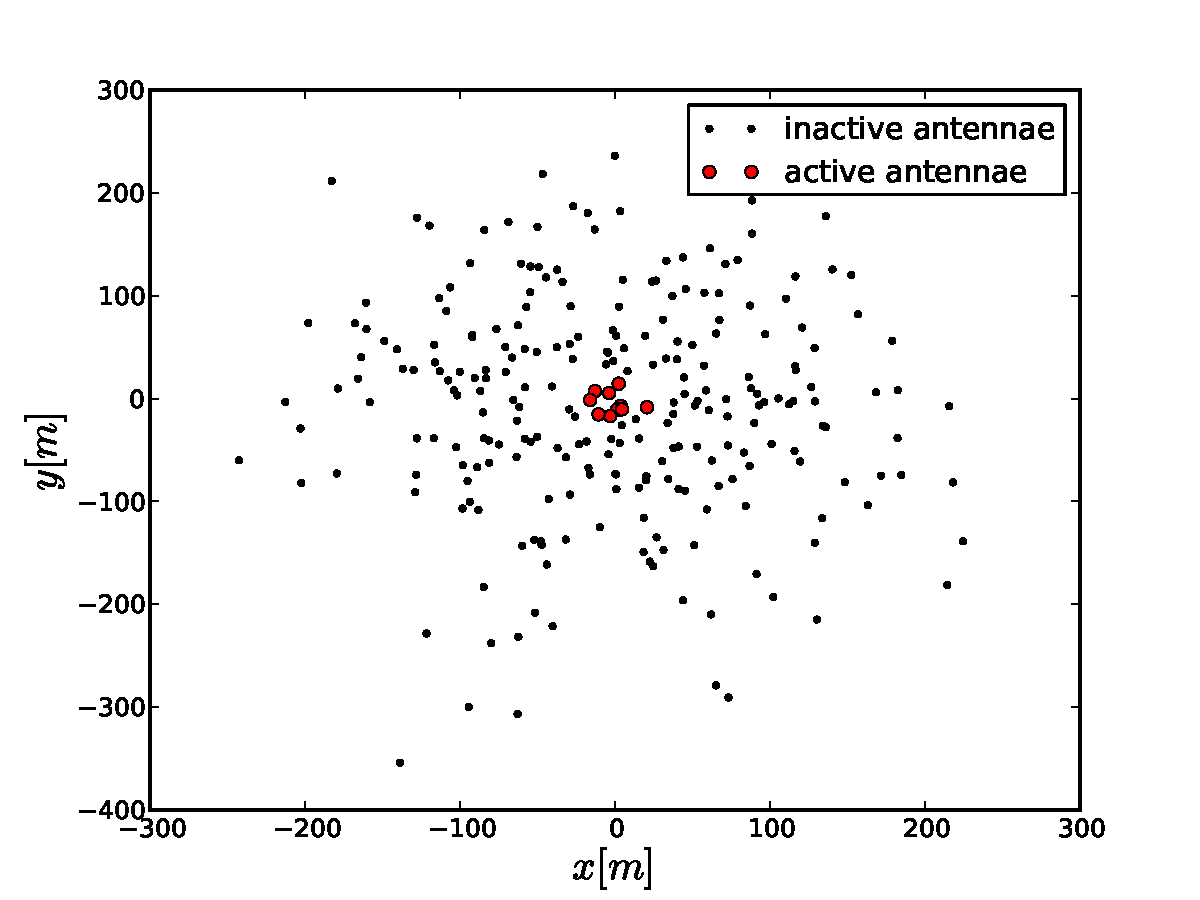
\includegraphics[width=0.5\textwidth]{10_closestantennae.pdf}
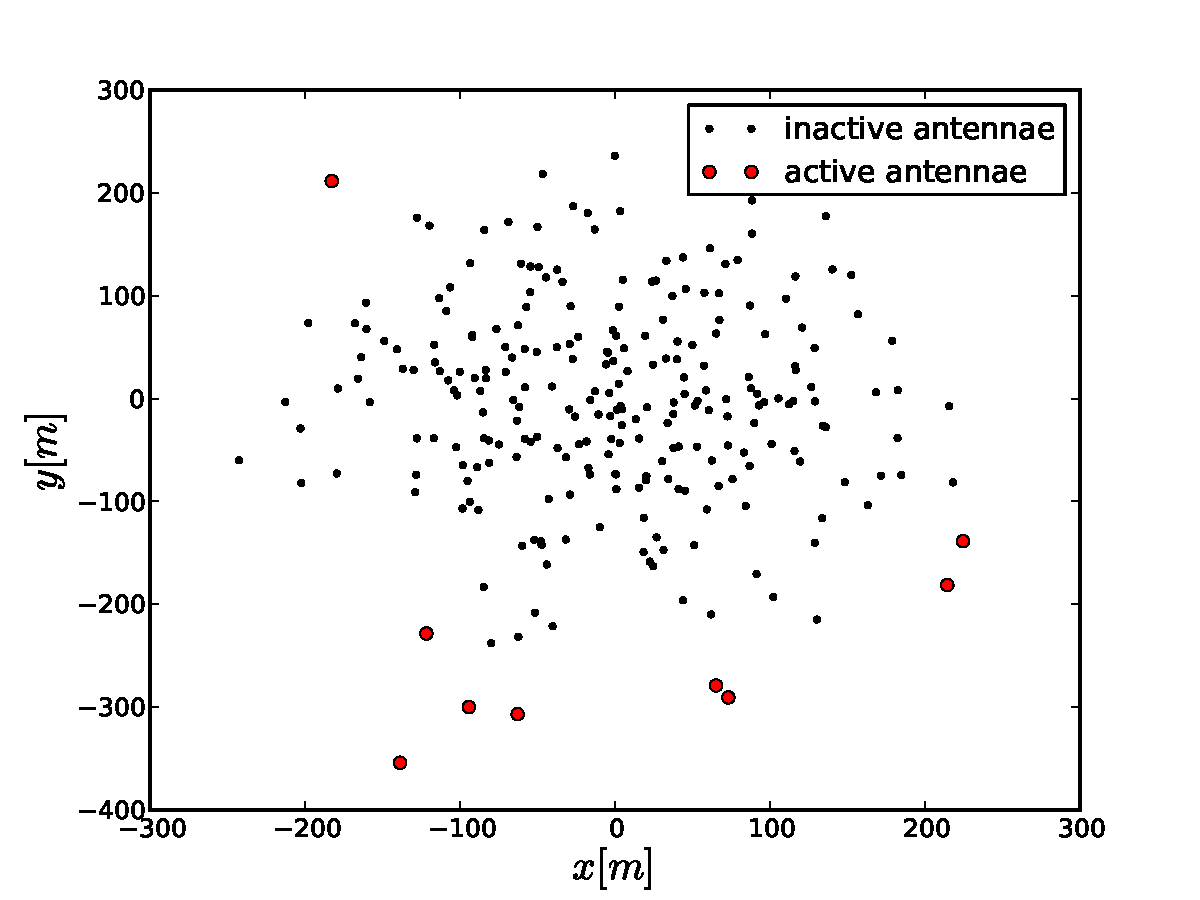
\includegraphics[width=0.5\textwidth]{10_farthestantennae.pdf}
}
\centerline{
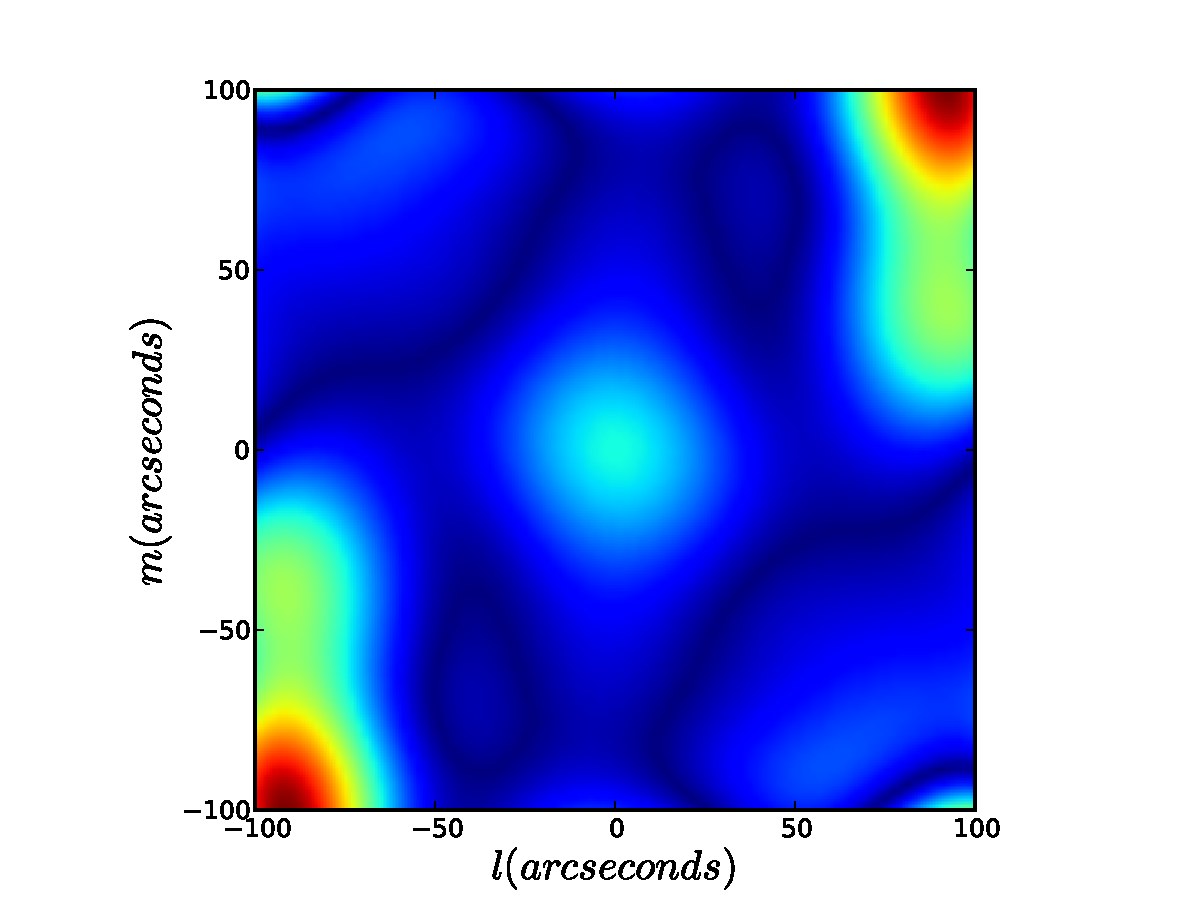
\includegraphics[width=0.5\textwidth]{DFT_image_10closest.pdf}
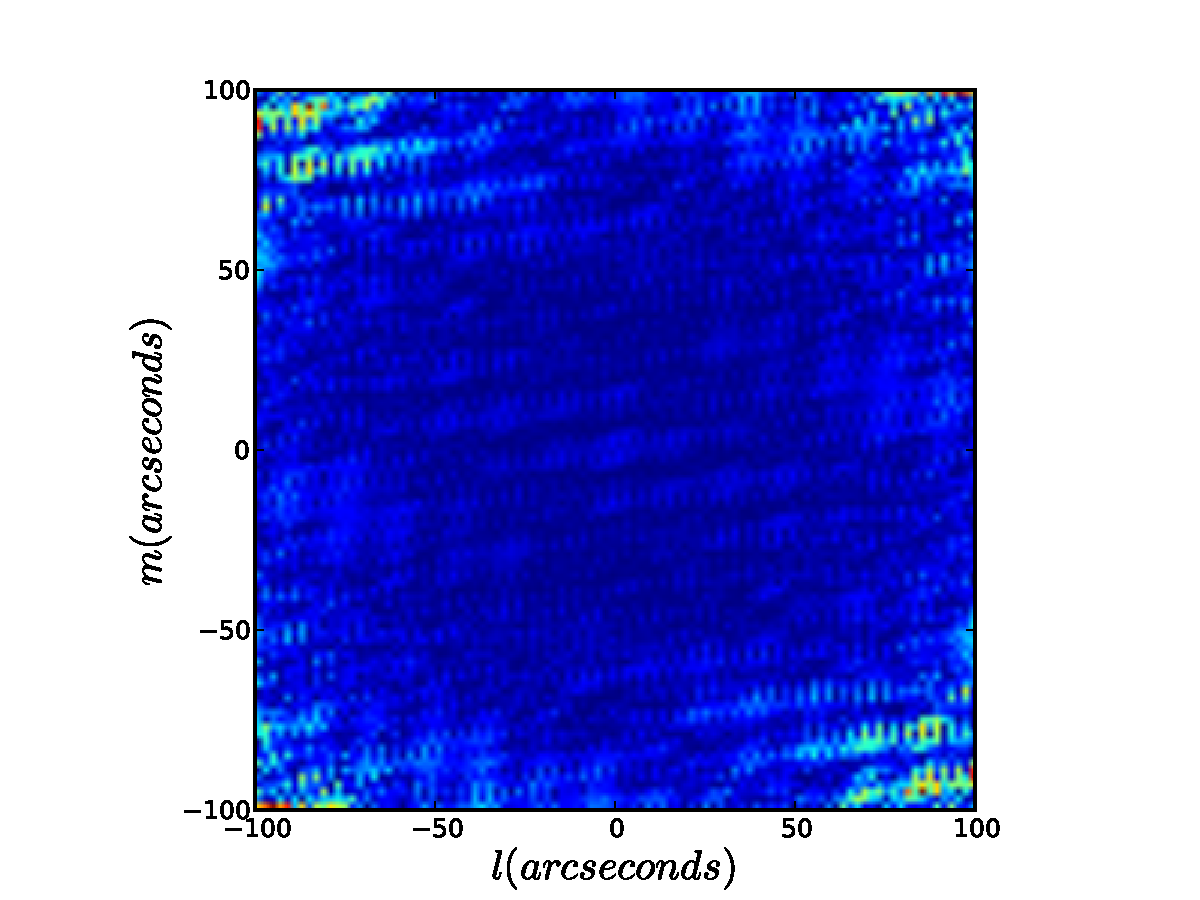
\includegraphics[width=0.5\textwidth]{DFT_image_10farthest.pdf}
}
\caption{Image created with a DFT using (left) $10$ closest and (right) $10$ farthest antennae. The top row shows the antennae positions, while the bottom row shows the corresponding image created.}
\label{fig:dft_results}
\end{figure}



\section{Imaging with an FFT}
Python's built-in FFT and inverse-FFT functions expect the input 
to be on an evenly spaced grid.  So to form an image from the 
measured visibilities using an FFT, we first had to place the 
visibilities on such a grid.  We created a 100$\times$100 grid in 
the $(u,v)$ plane.  For each measured $u$ and $v$ value, we found the 
grid $u$ and $v$ it was closest to using Python's \texttt{bisect\_left} 
function.  This function returns the location of where a given value 
would be inserted in a sorted array.  So, given a measured $u$ or $v$, 
the closest grid $u$ or $v$ is one of the elements on either side of 
where the measured value would be inserted into the grid.  Subtracting the 
measured value from each of these two elements gives which grid element 
element is closest.  Once each measured $(u,v)$ is assigned to a 
gridpoint in this way, the visibility at each gridpoint is defined 
to be the sum of all the measured visibilities assigned to that gridpoint.

The gridded visibilities are then use to form an image.  From Equation 
\ref{eq:vis3}, it is easy to see that intensity is given by:
\begin{equation}
I(l,m)=\frac{\hat{\mathcal{V}}(l,m)\sqrt{1-l^2-m^2}}{A(l,m)},
\end{equation}
where $\hat{\mathcal{V}}(l,m)$ is the inverse-FFT of the gridded 
visibilities.  The resulting image is shown in Figure \ref{fig:fft}.

\begin{figure}[!h]
\centering
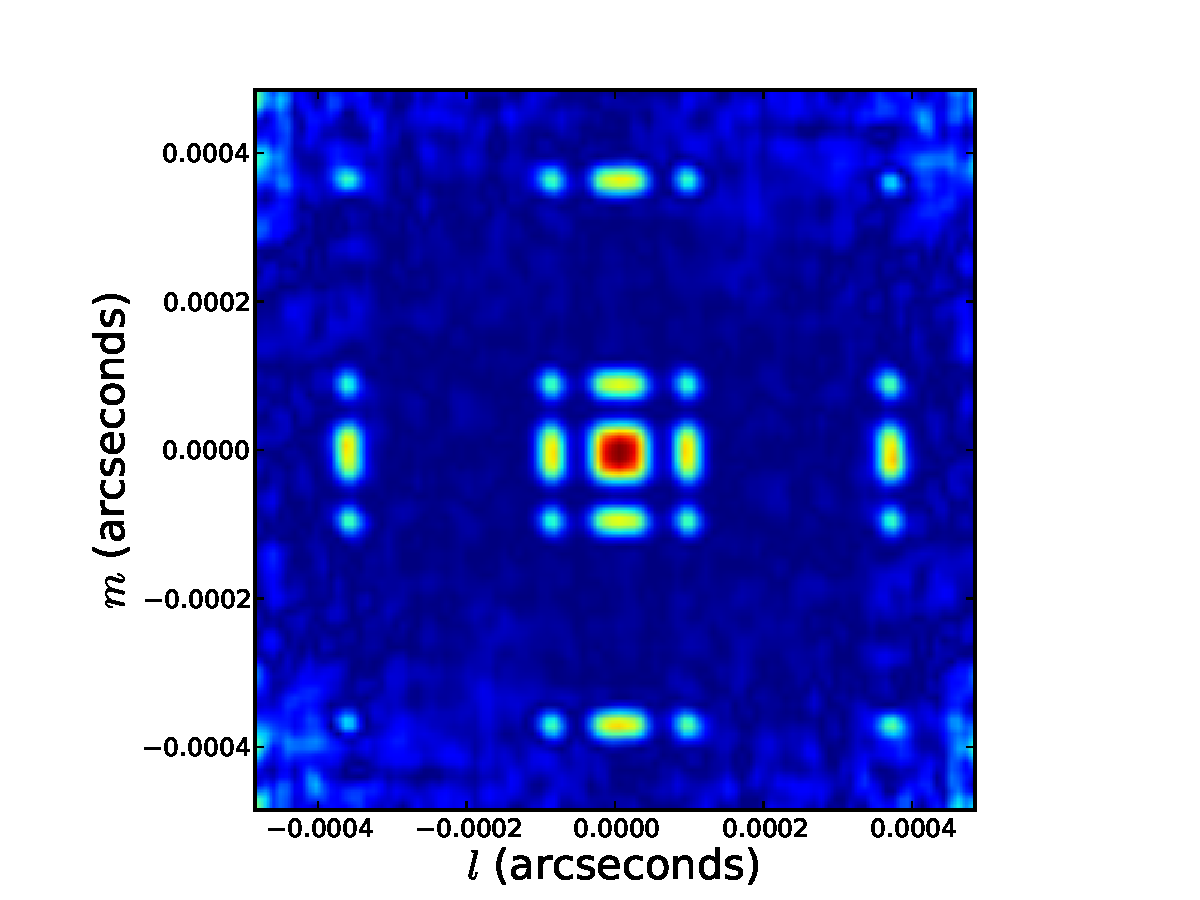
\includegraphics[width=0.5\textwidth]{FFT_Image.pdf}
\caption{Image created with an FFT using all 256 antennae.}
\label{fig:fft}
\end{figure}


\section{Discussion}
\subsection{Number of Antennae}

\subsection{Timing}
To test the performance of our DFT and FFT routines, we used Python's built-in 
timing capabilities to determine how long each routine takes for different 
numbers of antennae $N$.  The results are shown in Figures \ref{fig:DFTtime} and 
\ref{fig:FFTtime}.  The DFT routine has to loop through all $N(N-1)$ baselines 
to perform the Fourier transform.  So, for large $N$, the time required to 
run the DFT routine should go as $N^2$.  This matches what we observe.  On the 
other hand, Python's FFT algorithm runs in $\mathcal{O}(N\log N)$ time.  Figure 
\ref{fig:FFTtime} shows that, while there is some scatter to the fit, the time 
to run the routine follows an $N\log N$ proportionality reasonably well.  
The scatter may be due to small variations in the computer's performance in 
each run (note the scale), or due the the additional step in the FFT of 
gridding the data.  More important than the exact scaling is the fact that 
the FFT is much faster than the DFT.  In the interest of time, we only timed 
the DFT for up to 20 antennae.  Even using only 20 antennae, the DFT was nearly 
five times slower than the FFT using 250 antennae.

\begin{figure}[!h]
\centering
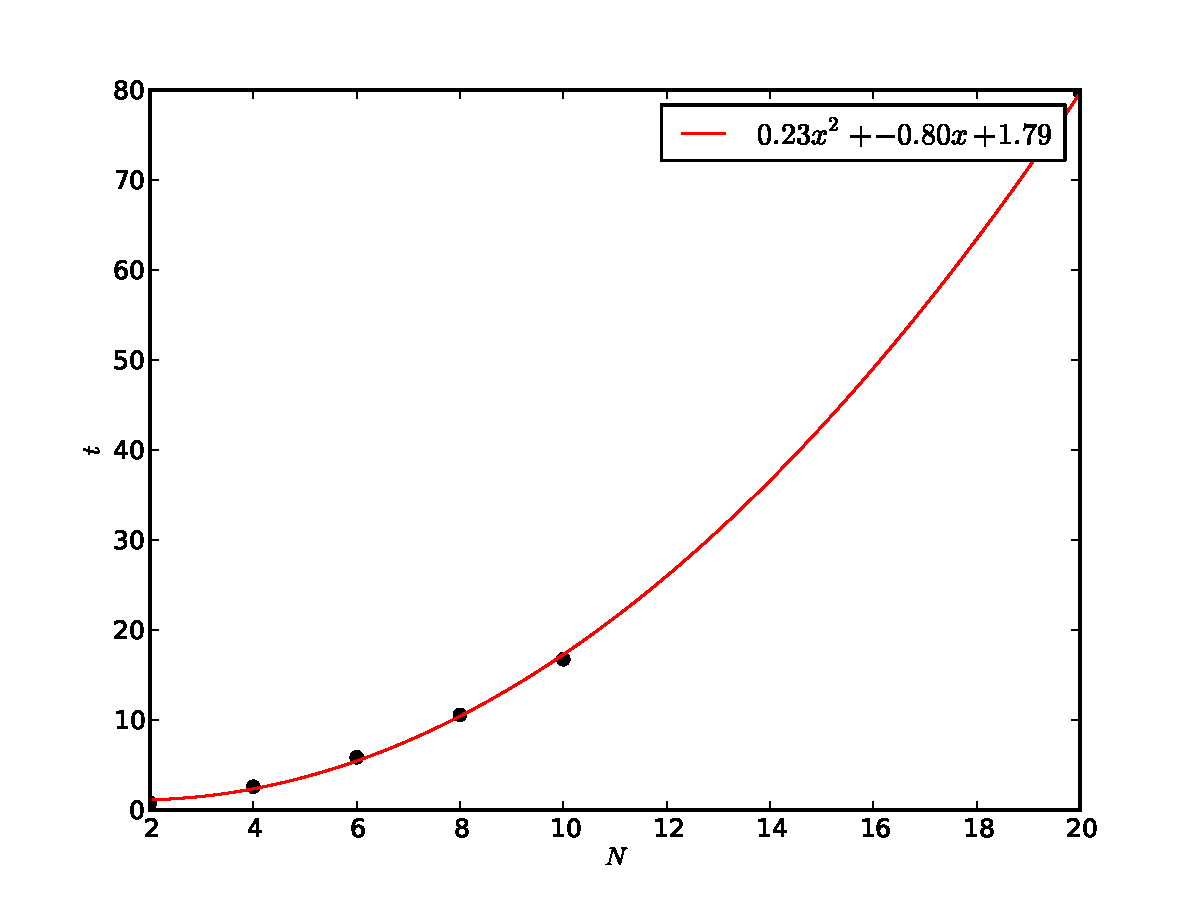
\includegraphics[width=0.5\textwidth]{DFT_image_timing.pdf}
\caption{Time (in seconds) required to run our DFT routine as a function of 
antenna number.  As expected, $t\propto N^2$.}
\label{fig:DFTtime}
\end{figure}

\begin{figure}[!h]
\centering
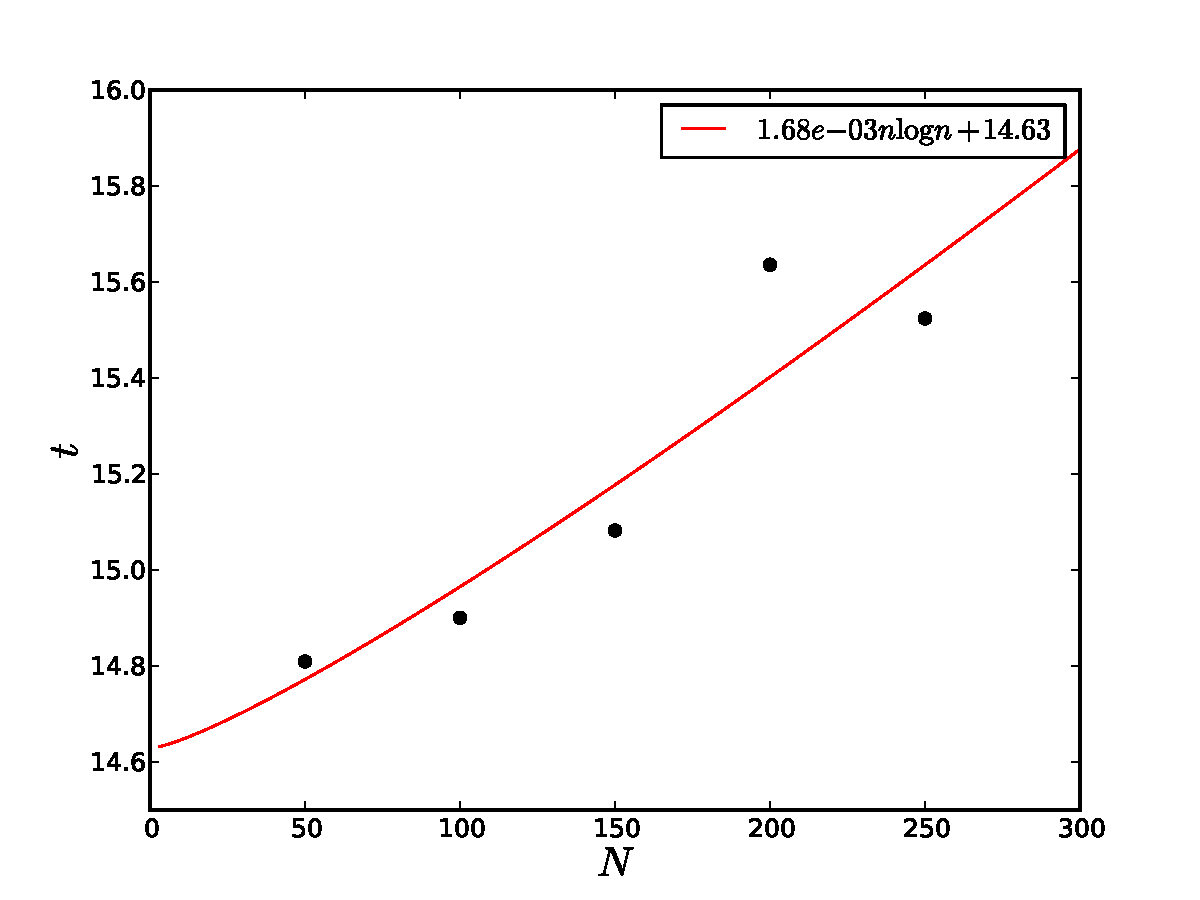
\includegraphics[width=0.5\textwidth]{FFT_image_timing.pdf}
\caption{Time (in seconds) required to run our FFT routine as a function of 
antenna number.  As expected, $t\propto N\log N$.  Also note that the FFT 
runs much more quickly than the DFT.}
\label{fig:FFTtime}
\end{figure}

\subsection{Gridding}
One of the key steps in performing an FFT of the visibilities is gridding.  
For this project, by adding all measured visibilities to the gridpoints 
to which they were assigned, we are giving equal weight to each 
measured visibility when computing the FFT.  This seems like a natural 
thing to do, but it does introduce possible problems.  If the radio array 
provides non-uniform $(u,v)$ coverage, extra weight will be given to 
certain gridpoints just because they have more measured 
visibilities around them.  For example, the Owens Valley LWA 
has 256 antennae within a 200 meter radius, providing over 
30,000 relatively short baselines.  To increase angular 
resolution, several new antennae are being built with baselines 
of 2 km.  If equal weighting were given to all measured visibilities, 
the few long baselines would be completely dominated by the 30,000 
shorter baselines, negating the increased resolution.  One way around 
this problem is to build additional antennae to more uniformly cover the 
$(u,v)$ plane.  However, this is often expensive and impractical, so instead, 
the visibilities from the shorter baselines can be given less weight than 
ones from the longer baselines.  This allows the longer baselines to 
increase the resolution of the array, but decreases its overall 
sensitivity due to the contribution of so many visibilities being decreased.


\end{document}

